\documentclass[a4paper,12pt]{article}

\pdfminorversion=4

\usepackage[left=2.5cm,top=2.5cm,right=2.5cm,bottom=2.5cm]{geometry}

\usepackage[T1]{fontenc}
\usepackage[spanish]{babel}
\usepackage[utf8]{inputenc}

\usepackage[pdftex, breaklinks=false, colorlinks=true, linkcolor=black, anchorcolor=black, urlcolor=blue, citecolor=red]{hyperref}
\usepackage{graphicx}
\usepackage{times}
\usepackage{inconsolata}
\usepackage{float}
\usepackage{minted}

\usemintedstyle[console]{vs}

\newminted[bashcode]{console}{} % tango vs
\newminted{python}{}


\usepackage{comandos}


\def \titulo{Amuse Bouche: Aplicación Android de visualización de recetas}
\def \autor{Alumno: Noelia Sales Montes\\Tutor: Manuel Palomo Duarte}
\def \fecha{Septiembre de 2016}

\usepackage{parskip}
\usepackage{abstract}

\begin{document}
\portada

\vspace{0.25cm}

\begin{abstract}
  \textbf{Amuse Bouche} es un proyecto que consiste en desarrollar una
  aplicación móvil para la visualización de recetas de cocina licenciada bajo
  software libre, acompañada de su correspondiente API para el manejo de datos.

  La parte básica de la aplicación permitirá visualizar dichas recetas,
  agregándole un sentido semántico a los ingredientes y a la propia receta en sí
  (mediante etiquetado, categorización o datos tomados del usuario o del
  contexto).

  Cada uno de los pasos de la receta podrá contener, además de la propia descripción
  textual, elementos gráficos (imágenes o videos) y un tiempo definido, gracias al
  cual se podrá activar un cronómetro de tiempo de espera.

  Además de poder acceder a otros datos básicos referentes a la propia receta, los
  usuarios podrán votarlas mediante un sistema de puntuación.

  También se le dará un caracter internacional a la aplicación, puesto que las
  recetas tendrán definido el idioma en el cual están escritas. Así cada usuario
  podrá leer las recetas del lenguaje que le sea relevantes. \\

  \textbf{Palabras clave:} app, receta, ingrediente, dieta, Android, Python,
Django, API, Servidor.

\end{abstract}


% \vspace{0.5cm}

\section{Introducción}

\subsection{Contexto y motivación}

Los móviles y tabletas son parte habitual en la vida diaria de las personas, por
lo que cada día surgen nuevas aplicaciones para mejorar cualquiera de las
acciones que tenemos que llevar a cabo a diario. Esto incluye la cocina.

Son multitud las aplicaciones creadas tanto para los amantes de esta actividad,
como para aquellos a los que esto les aborrece y necesitan de un impulso para
manejarse mejor. Son habituales las aplicaciones con recetarios variados, aunque
la mayoría cerrados a actualizaciones externas. Menos son las que incluyen la
capacidad de permitir a sus usuarios subir y compartir sus propias recetas.

De esto se extrae la necesidad de que existan aplicaciones para facilitar la
lectura y comprensión de las diferentes recetas de cocina.

A este contexto se suma la motivación personal de la autora quien, estando
habituada a cocinar a diario y a buscar nuevas recetas para poder realizar, se
encontró con la problemática de que al utilizar el dispositivo para ir
leyendo los pasos de la receta, dejaba de lado las labores de la cocina
o llegaba a poner en peligro el dispositivo. Ante esto, surgía la necesidad de
que el dispositivo no solo indique al usuario los pasos a seguir, sino que el
usuario pueda darle órdenes a distancia de forma que no tenga que dejar lo que
esté haciendo.


\subsection{Objetivos}

Los principales objetivos a alcanzar son los siguientes:

\begin{itemize}
\item Crear una aplicación móvil de acceso público que permita la visualización
  de recetas de cocina, su lectura automática y la recepción de órdenes del
  usuario.
\item Permitir la creación y la subida de nuevas recetas para poder compartirlas.
\item Habilitar la categorización de dichas recetas a través de sus propios
  ingredientes o según otros criterios, para facilitar su búsqueda, sobre todo
  de cara a personas alérgicas o intolerantes.
\item Permitir mostrar imágenes, videos o utilizar un cronómetro en cada paso
  de la receta.
\item Permitir que se suban las recetas en varios idiomas.
\item Permitir la socialización por medio de comentarios y votaciones sobre las
  recetas.
\item Ampliar los conocimientos sobre desarrollo de aplicaciones móviles (en
  particular, en plataformas Android) y sobre desarrollo de una API REST.
\item Investigar y conocer más información acerca del mundo de la cocina.
\item Permitir ampliaciones y modificaciones a futuro sobre la aplicación.
\end{itemize}


\subsection{Planificación}

El proyecto se ha desarrollado siguiendo un calendario basado en fases,
utilizando un modelo de desarrollo iterativo incremental. En la
tabla~\ref{tab:estimacion_tiempo} se presenta a continuación una comparación por
fases de los plazos estimados frente a los plazos reales tras la conclusión del
proyecto.

\begin{table}[hbtp]
  \centering
  \begin{tabular}{|l|r|r|}
    \hline
    \textbf{Iteración} & \textbf{Tiempo estimado} & \textbf{Tiempo real} \\
    \hline
    Planificación & 56 horas & 77 horas \\
    \hline
    Aprendizaje & 224 horas & 242 horas \\
    \hline
    Diseño visual & 56 horas & 22 horas \\
    \hline
    Desarrollo API & 128 horas & 110 horas \\
    \hline
    Desarrollo app & 128 horas & 132 horas \\
    \hline
    Ampliación API & 168 horas & 88 horas \\
    \hline
    Ampliación app & 216 horas & 222 horas \\
    \hline
    Despliegue & 32 horas & 26 horas \\
    \hline
    Resolución de \textit{bugs} & 160 horas & 152 horas \\
    \hline
    Documentación & 80 horas & 65 horas \\
    \hline
    \textbf{Total} & 1249 horas & 1136 horas \\
    \hline
  \end{tabular}
  \caption{Comparación de la estimación con los tiempos reales}
  \label{tab:estimacion_tiempo}
\end{table}


\subsubsection{Primera iteración: preparación previa}
\label{sec:primera_iteracion}

Antes de abarcar el desarrollo, era necesario definir los requisitos que tendría
el sistema y dividirlos en niveles de prioridad. Una vez bien definidos, se
estudiaron y definieron los lenguajes y \textit{frameworks} a utilizar durante
el desarrollo de este y se dedicó tiempo a aprender cómo funcionaban.

Por último, se empezó a definir el diseño visual de aplicación, tanto el
logotipo como la paleta de colores y demás detalles involucrados.


\subsubsection{Segunda iteración: desarrollo de la base de la API}
\label{sec:segunda_iteracion}

En esta etapa se define el modelo de datos básico a abarcar para los requisitos
más prioritarios (basados en la visualización básica de recetas). Además, se
creó el proyecto de Django y se construyó la estructura básica de modelos,
serializadores y vistas, con la funcionalidad CRUD necesaria para obtener la
información requerida.


\subsubsection{Tercera iteración: desarrollo de la base de la aplicación móvil}
\label{sec:tercera_iteracion}

Tras construir la base de la API, se empezó a desarrollar la aplicación Android.
Se construyó la estructura del proyecto y se implementaron las clases y métodos
necesarios, así como las \textit{actividades} y \textit{fragmentos} que forman
las vistas iniciales. Estas vistas eran las referentes a la vista inicial (el
listado de recetas) y la vista de detalle de una receta concreta.


\subsubsection{Cuarta iteración: ampliación de la API}
\label{sec:cuarta_iteracion}

Una vez la API y la aplicación eran estables y cumplían los requisitos más
prioritarios, se decidió ampliar la API para abarcar el resto de requisitos. Se
añadieron los atributos y métodos necesarios para permitir el filtrado de
recetas, lo cual era necesario para abarcar la semántica de las recetas y la
internacionalización. También se añadió la funcionalidad necesaria para permitir
comentar y puntuar las recetas.


\subsubsection{Quinta iteración: ampliación de la aplicación móvil}
\label{sec:quinta_iteracion}

Tras ampliar la API, se actualizaron los métodos que trabajaban con la base de
datos para añadir los nuevos atributos. También se añadieron nuevas vistas a la
app, como la vista de filtrado y la vista de edición, así
como la vista de \textit{login}.

\subsubsection{Sexta iteración: pruebas finales y despliegue}
\label{sec:sexta_iteracion}

Para finalizar, hubo que realizar el plan de pruebas de forma más estricta para
encontrar los \textit{bugs} que surgieran y corregirlos. Este plan se llevó a
cabo una vez realizado el despliegue de la API en un servidor en producción, para
asegurar que funcionara en las mismas condiciones en las que se encontrarán los
usuarios finales. En esta etapa también se documentó esta memoria y se afinaron
los detalles finales.



\section{Descripción general}

\textbf{Amuse Bouche} se modela como una aplicación móvil para la visualización
de recetas. Los usuarios tendrán la posibilidad de crear y editar sus recetas y
elegir la opción de compartirlas con los demás usuarios, a través de una API.
También podrán visualizar todos los detalles de cada receta y utilizar el modo
de lectura y captura de órdenes para cocinar a medida que el dispositivo les
informa de cada paso a seguir.

Se incluyen otras funcionalidades como la capacidad de que las recetas se
encuentren en varios idiomas o la categorización de dichas recetas para poder
filtrarlas en función de sus alérgenos, entre otras.


\subsection{API}

La API se encarga de proporcionar todos los datos a la aplicación móvil, aunque
esta puede utilizarse perfectamente de forma independiente. Esta API proporciona
una serie de \textit{endpoints}, los cuales se corresponden con los siguientes
modelos de datos:

\begin{figure}[H]
  \centering
  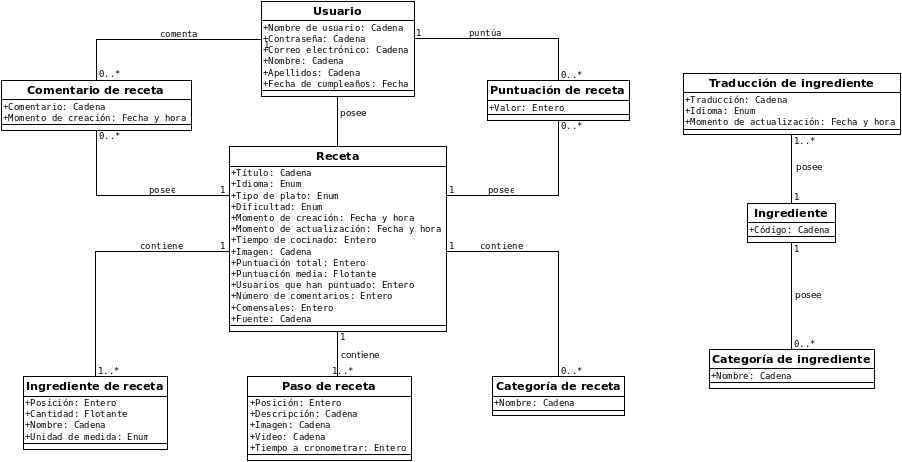
\includegraphics[width=\textwidth]{./img/diagrama_clases_conceptuales}
  \caption{Modelo conceptual}
  \label{fig:modelo-conceptual}
\end{figure}

\begin{itemize}
\item \textit{Usuario}: Representa un usuario de la aplicación, que está relacionado
  con varios modelos, como el de ``Receta''.
\item \textit{Receta}: Representa una receta de cocina con su título, el idioma
  en que está escrita o la dificultad de realizarla. Está directamente
  relacionada con los modelos de ``Ingrediente de receta'', ``Paso de receta'' y
  ``Categoría de receta''.
\item \textit{Puntuación}: Representa una valoración dada por un usuario sobre
  una receta.
\item \textit{Comentario}: Representa un comentario dado por un usuario sobre
  una receta.
\item \textit{Ingrediente}: Representa un ingrediente categorizado. Está
  directamente relacionado con los modelos de ``Categoría de ingrediente'' y
  ``Traducción de ingrediente''.
\end{itemize}


\subsubsection{Aplicación móvil}

El producto principal dentro de este proyecto es una aplicación nativa para el
sistema operativo móvil Android que ofrece a los usuarios las funcionalidades que
se han comentado previamente.

El sistema se ha construido conforme al estándar de
Android,\cite{learning-android} por lo que la organización principal del código
se divide en los siguientes componentes:
\begin{itemize}
\item \textsc{Actividades}: Clases que se encargan de crear una ventana donde mostrar una
  interfaz de usuario. Las actividades principales son las de la pantalla de
  carga inicial, la de la actividad principal (que conecta las pantallas de
  listado de recetas, login, registro y usuario conectado, configuración e
  información), la del detalle de una receta (que contiene todo el sistema de
  lectura automática) y de edición de una receta.
\item \textsc{Adaptadores}: Clases que sirven de puente entre una vista y los datos que
  la conforman, como puede ser por ejemplo el adaptador de las celdas del
  \textit{grid} de la vista de listado de recetas.
\item \textsc{Datos}: Clases de datos e interfaces con la base de datos (denominadas
  \textit{contracts}. Aquí se definen todas las clases del modelo de datos
  que se corresponde casi idénticamente con el de la API, aunque algo más
  simplificado.
\item \textsc{Diálogos}: Clases con las ventanas que aparecen para hacer que el usuario
  tome una decisión o introduzca información adicional.
\item \textsc{Fragmentos}: Clases que reflejan una parte de la interfaz gráfica o de un
  comportamiento que puede incluirse dentro de una actividad. Por ejemplo, en
  el caso de la actividad de la patalla de detalle, encontramos 4 fragmentos
  incluidos en ella, para cada una de las pestañas que contiene (datos generales,
  ingredientes, preparación y comentarios).
\item \textsc{Servicios y manejadores}: Clases que intervienen para facilitar al usuario
  el usuario de diversos elementos o bibliotecas, como por ejemplo la realización
  de peticiones a la API o las llamadas a la base de datos.
\item Componentes personalizados de la interfaz gráfica.
\end{itemize}

\begin{figure}[H]
  \centering
  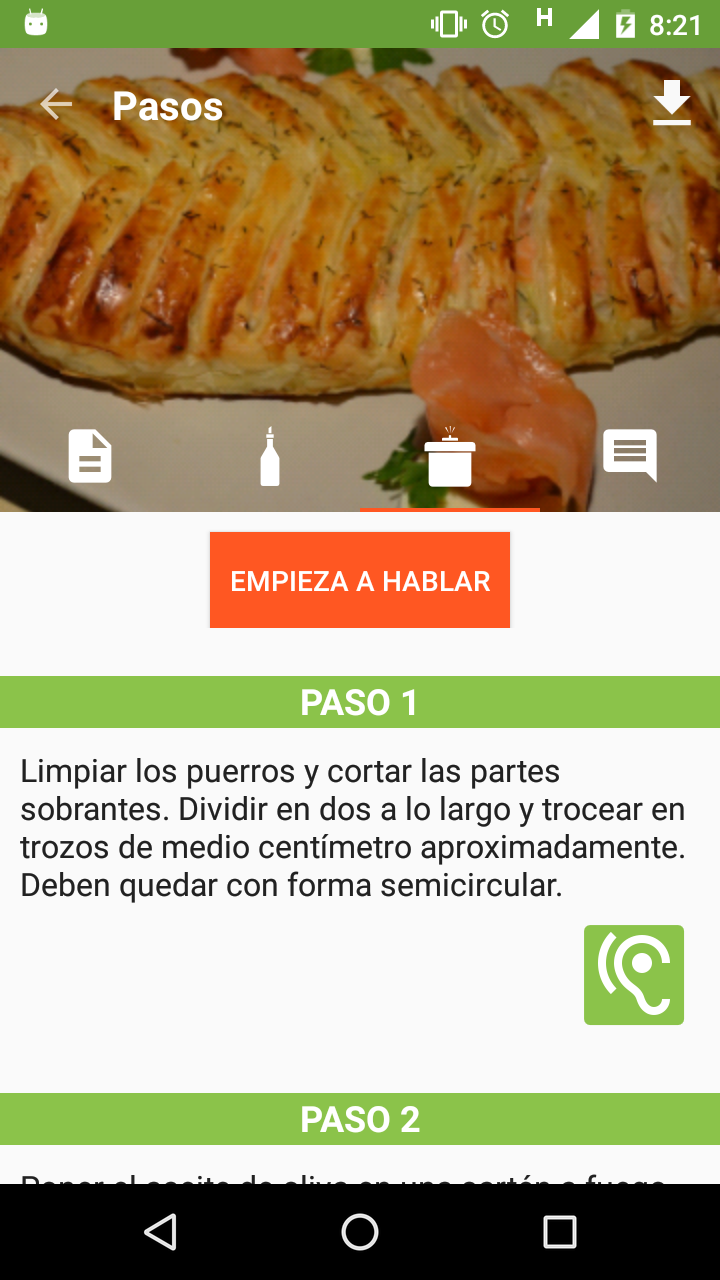
\includegraphics[width=0.4\textwidth]{./img/captura}
  \caption{Captura de la aplicación móvil}
  \label{fig:captura}
\end{figure}

Todas estas clases se completan con los recursos adicionales necesarios, como
pueden ser los \textit{layouts} que definen la interfaz gráfica de un fragmento
o de una actividad, las imágenes e iconos utilizados en la aplicación o la
definición de datos como cadenas internacionalizadas o estilos.


\section{Desarrollo del sistema}

Durante el desarrollo de este proyecto surgiron varias cuestiones importantes
a dirimir durante la implementación, debido a la cantidad de tecnologías y
objetivos que se pretendian conseguir. Una de las cuestiones más importantes es
la que se refleja a continuación.

\subsection{Detalle de implementación de la categorización de ingredientes}

La idea original para este sistema es que fuera completamente automático. Es
decir, que fuera capaz de detectar dinámicamente en función del nombre de un
ingrediente si es alérgeno o no.

Para ello, se intentaron utilizar proyectos que manejan información semántica,
como dbpedia. Se hicieron varias pruebas trabajando con consultas sobre esa
información, probando en ambos sentidos: obteniendo información de un ingrediente
y buscando si estaba categorizado como alérgeno y  obtenido información de una
categoría alérgena (como, por ejemplo, el marisco) y buscando si aparecían
los ingredientes que formaban parte de dicha categoría. Un ejemplo de dichas
consultas es el siguiente:

\begin{bashcode}
PREFIX dcterms: <http://purl.org/dc/terms/>
select * where{
  ?marisco dcterms:subject <http://es.dbpedia.org/resource/Categoría:Marisco> .
}
\end{bashcode}

Sin embargo, la información que proporcionaban estas consultas era inconsistente
de un ingrediente a otro y no permitía una forma automatizada de filtrar dicha
información.

Teniendo en cuenta que, bajo la premisa inicial, es muy importante que la
aplicación no de un falso positivo, es decir, \textbf{nunca} debe filtrar como
``APTA PARA CELÍACOS'' una receta que no lo es. Por tanto, fue necesario
implementar un sistema de ingredientes categorizados integrado dentro de la
propia API.

Se incluyeron clases específicas para manejar los datos de los ingredientes y
sus categorías asociadas (los alérgenos). Además, teniendo en cuenta que la
aplicación móvil debía ser multiidioma, añadimos la capacidad de traducir cada
ingrediente a cada idioma. Así, tuvieron que añadirse los modelos
\texttt{Ingredient}, \texttt{IngredientCategory} y \texttt{TranslatedIngredient},
según ya se vio en el capítulo~\ref{chap:diseno}, en la
sección~\ref{sec:diseno-fisico-datos}.

\begin{minted}{python}
# Generic ingredients
class Ingredient(models.Model):
    code = models.CharField(max_length=100)

class TranslatedIngredient(models.Model):
    ingredient = models.ForeignKey(Ingredient, related_name='translations')
    translation = models.CharField(max_length=100)
    language = models.CharField(choices=LANGUAGE_CHOICES, default='es',
        max_length=10)
    timestamp = models.DateTimeField(auto_now=True)

class IngredientCategory(models.Model):
    ingredient = models.ForeignKey(Ingredient, related_name='categories')
    name = models.CharField(max_length=100)
\end{minted}

Al entrar en la aplicación móvil, se descargan todos los ingredientes del
idioma seleccionado. Inicialmente se descargan todos y se guarda la fecha, para
posteriormente descargar tan sólo aquellos que se hayan actualizado a posteriori.

Cuando un usuario va a crear o editar una receta, se utilizan estos ingredientes
almacenados para comprobar qué categorías tienes asociadas y añadirlas
automáticamente a la receta conforme se vayan incluyendo los ingredientes. En
caso de que se añada un ingrediente que no existe en la base de datos, se añade
la categoría de ``SIN CATEGORIZAR'', para asegurar que sea revisada manualmente.

El siguiente código forma parte del flujo comentado:

\begin{minted}{java}
/**
 * Add category for a new ingredient that has been set.
 * Search the ingredient categories and check if they have been added
 * yet. Otherwise, add them.
 *
 * @param name Ingredient name that has been added.
 */
private void addCategoryForIngredient(String name) {
    if (mDatabaseHelper.existIngredient(name)) {
        // If ingredient exists in database, we add all its categories
        //to the recipe
        Ingredient ing = mDatabaseHelper.getIngredientByTranslation(name);

        ArrayList<String> categories = new ArrayList<>(
            Arrays.asList(ing.getCategories().split(
                Pattern.quote(Ingredient.CATEGORY_SEPARATOR))));

        for (int c = 0; c < categories.size(); c++) {
            boolean found = false;

            for (int ci = 0; ci < mEditionActivity.getRecipe().
                getCategories().size(); ci++) {
                if (categories.get(c).equals(mEditionActivity.getRecipe()
                    .getCategories().get(ci).getName())) {
                    found = true;
                }
            }

            if (!found) {
                // Add category to recipe
                mEditionActivity.getRecipe().getCategories().add(
                    new RecipeCategory(categories.get(c)));

                // Add category to forced recipes
                mEditionActivity.getForcedCategories().add(categories.get(c));
            }
        }
    } else {
        // If ingredient doesn't exist in database, we add
        // UNCATEGORIZED category
        boolean found = false;

        for (RecipeCategory c :
             mEditionActivity.getRecipe().getCategories()) {
            if (c.getName().equals(RecipeCategory.CATEGORY_UNCATEGORIZED)) {
                found = true;
            }
        }

        if (!found) {
            // Add category to recipe
            mEditionActivity.getRecipe().getCategories().add(
                new RecipeCategory(RecipeCategory.CATEGORY_UNCATEGORIZED));

            // Add category to forced recipes
            mEditionActivity.getForcedCategories().add(
                RecipeCategory.CATEGORY_UNCATEGORIZED);
        }
    }
}
\end{minted}

Se ha intentado buscar otros métodos que automaticen esto, pero de momento no se
ha encontrado ninguno que no ponga en riesgo que aparezcan falsos positivos.


\subsection{Verificación y pruebas}

Para comprobar la corrección del software se han llevado a cabo varios procesos
de verificación y baterías de pruebas a distintos niveles.

\subsubsection{Pruebas funcionales}

Se definió un plan de pruebas completo para cada bloque funcional de la
aplicación móvil, cuya verificación asegura que el sistema cumple con todos los
requisitos establecidos. En cada iteración, las pruebas se ejecutaron sobre el
entorno de pruebas desplegado con Vagrant y se conectaron dispositivos para
comprobar cómo se comportaba en condiciones reales.

\subsubsection{Pruebas no funcionales}

Con objeto de verificar aspectos del proyecto más allá de su funcionalidad, las
pruebas no funcionales cubrieron bastantes frentes distintos. En particular:

\begin{itemize}
\item Se llevaron a cabo pruebas de \textbf{seguridad}, centradas principalmente
  en verificar que la información de los usuarios y las áreas privadas de la API
  eran seguras.
\item Se aseguró la \textbf{calidad del código}, mediante la utilización de
  revisadores de código automáticos para asegurar que cumplía con los estándares
  de codificación.
\end{itemize}


\section{Conclusiones y difusión}

Tras la realización del proyecto se han dado unos resultados que dan lugar a
conclusiones, tanto personales como públicas, que se reflejan a continuación.

\subsection{Objetivos cumplidos}

Se han completado con éxito todos los objetivos presentes desde el inico del
proyecto. Concretamente:

\begin{itemize}
\item Se ha creado una aplicación de acceso público con la que los usuarios
  puede crear sus propias recetas y compartirlas. Está disponible en Google
  Play (falta enlace).
\item Dicha aplicación permite todos los requisitos que se elicitaron
  inicialmente: listado de recetas, compartir recetas, categorización y filtrado,
  varios idiomas y socialización.
\item El sistema se ha desarrollado de tal forma que es fácilmente ampliable,
  tanto la API como la aplicación Android.
\end{itemize}

Además de completar los objetivos funcionales, se han completado aquellos
transversales, mucho más personales. He ampliado mucho mis conocimientos en las
tecnologías utilizadas, hasta tal punto que en mi trabajo ya he podido
participar en proyectos Android gracias a la experiencia conseguida y
demostrada. También me ha servido para ampliar mis conocimientos culinarios,
llegando incluso a abrir un blog de cocina personal,\cite{noeliarcado} fuente
inicial y principal de las recetas publicadas en la aplicación.

\subsection{Conclusiones personales}

\textit{Amuse Bouche} es un proyecto personal que ha surgido para suplir una
necesidad propia, real y compartida por muchas personas, y que ha cumplido su
objetivo, aunque todavía queda mucho por hacer. La aplicación es capaz de
solventar los problemas indicados en la sección~\ref{sec:situacion-actual}, por
lo que estoy muy satisfecha con el trabajo realizado.

\subsubsection{Lecciones aprendidas}

Este proyecto puede parecer algo simple si lo separamos en cada una de sus
funcionalidades por separado, pero el querer reunir todas ellas en un mismo
sistema ha sido complejo y duro, bastante más de lo que parece desde una
perspectiva externa.

Como aspecto positivo, he tenido la oportunidad de trabajar con tecnologías
actuales y bien estructuradas, con las cuales no me importaría volver a trabajar
en un futuro.

\bibliographystyle{hispa-annote}
\bibliography{bibliografia}

\vspace{0.75cm}

\begin{center}
  {\footnotesize Este documento se halla bajo la licencia FDL de GNU (Free
    Documentation License)\\ \url{http://www.gnu.org/licenses/fdl.html} }   
\end{center}

\end{document}
